\subsection{Setup Gitolite}

\initmarginpar{%

\includegraphics[width=\marginparwidth]{git_logo}
\begin{flushright}
\scriptsize{Git Logo, \mbox{CC BY 3.0 Unported,} \mbox{Author Jason Long,} \url{http://twitter.com/jasonlong}}%
\end{flushright}}

\begin{figure}[htp]
\centering
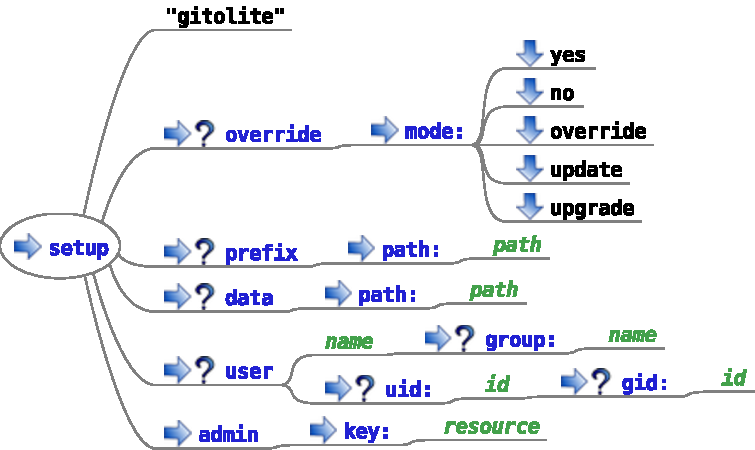
\includegraphics[width=0.7\textwidth]{source_setup_gitolite}
\label{fig:source_setup_gitolite}
\caption{Gitolite Statements}
\end{figure}

%% setup gitolite
\TheStatement[source:setup:gitolite]{setup "gitolite"}
\TheStatement*[source!setup!gitolite]{setup "gitolite", \{ override prefix data user admin \}}

Installs and configures the Gitolite\footnote{\url{http://gitolite.com/}} 
source code management service.

\begin{lstlisting}[style=Java]
source {
    setup "gitolite", {
        ...
    }
}
\end{lstlisting}

%% override
\TheStatement[source:setup:gitolite:override]{override}
\TheStatement*[source!setup!gitolite!override]{override \Arg{mode}}

Optionally, sets the override \Arg{mode} that determines what should be done if the
service was already installed inside the prefix path. The override mode can be
\begin{compactitem}
\item \code{no, OverrideMode\#no}, no update of the existing service;
\item \code{yes, OverrideMode\#override}, override the existing service;
\item \code{OverrideMode\#update}, Update the existing service, only if the 
new version is greater or equals to the current installed version, 
skip installation otherwise;
\item \code{OverrideMode\#upgrade}, Update the existing service, only if the 
new version is greater to the current installed version, 
skip installation otherwise.
\end{compactitem}

\begin{lstlisting}[style=Java]
source {
    setup "gitolite", {
        override mode: OverrideMode.override
    }
}
\end{lstlisting}

%% prefix
\TheStatement[source:setup:gitolite:prefix]{prefix}
\TheStatement*[source!setup!gitolite!prefix]{prefix path: \Arg{path}}

Optionally, sets the service prefix \Arg{path}, that is, the path to where the service
will be installed.

\begin{lstlisting}[style=Java]
source {
    setup "gitolite", {
        prefix path: "/usr/local/gitosis"
    }
}
\end{lstlisting}

%% data
\TheStatement[source:setup:gitolite:data]{data}
\TheStatement*[source!setup!gitolite!data]{data path: \Arg{path}}

Optionally, sets the service data \Arg{path}, that is, the path where the repositories
are located.

\begin{lstlisting}[style=Java]
source {
    setup "gitolite", {
        data path: "/usr/local/gitosis"
    }
}
\end{lstlisting}

%% user
\TheStatement[source:setup:gitolite:user]{user}
\TheStatement*[source!setup!gitolite!user]{user \Arg{name} [, group: \Arg{name}] [, uid: \Arg{id}] [, gid: \Arg{id}]}

Optionally, sets the service local user \Arg{name}, the service local user 
group \Arg{name}, the user \Arg{id} and the group \Arg{id}, that is the 
owner of new created repositories.

\begin{lstlisting}[style=Java]
source {
    setup "gitolite", {
        user "git", group: "git", uid: 99, gid: 99
    }
}
\end{lstlisting}

%% admin
\TheStatement[source:setup:gitolite:admin]{admin}
\TheStatement*[source!setup!gitolite!admin]{admin key: \Arg{resource}}

Sets the administrator public key \Arg{resource}.

\begin{lstlisting}[style=Java]
source {
    setup "gitolite", {
        admin key: "yourname.pub"
    }
}
\end{lstlisting}
